\documentclass[conference]{IEEEtran}
\IEEEoverridecommandlockouts
% The preceding line is only needed to identify funding in the first footnote. If that is unneeded, please comment it out.
\usepackage{cite}
\usepackage{amsmath,amssymb,amsfonts}
\usepackage{algorithmic}
\usepackage{graphicx}
\usepackage{textcomp}
\usepackage{xcolor}
\def\BibTeX{{\rm B\kern-.05em{\sc i\kern-.025em b}\kern-.08em
    T\kern-.1667em\lower.7ex\hbox{E}\kern-.125emX}}
\begin{document}

\title{A Comparative Study of Monolithic and Modular Architectures in a Dataset Driven Case Tracking Web Application\\
% {\footnotesize \textsuperscript{*}Note: Sub-titles are not captured in Xplore and
% should not be used}
% \thanks{Identify applicable funding agency here. If none, delete this.}
}

\author{\IEEEauthorblockN{Mireya Francesca Vella}
\IEEEauthorblockA{\textit{Institute of Information and Communication Technology} \\
\textit{Malta College of Arts, Science and Technology}\\
Paola, Malta \\
mireya.vella.i85114@mcast.edu.mt}
}

\maketitle

\begin{abstract}
This document is a model and instructions for \LaTeX.
This and the IEEEtran.cls file define the components of your paper [title, text, heads, etc.]. *CRITICAL: Do Not Use Symbols, Special Characters, Footnotes, 
or Math in Paper Title or Abstract.
\end{abstract}

\begin{IEEEkeywords}
component, formatting, style, styling, insert
\end{IEEEkeywords}

\section{Introduction}


\subsection{Description of Theme and Topic Rationale}
Backend architecture choices influence how easily a system can be changed, tested, and kept stable over time. In practice, teams often debate whether to keep an application as a monolith or to introduce stronger internal separation through modular or layered design. A monolithic backend can be simpler to build initially, but it can become harder to maintain as features and business rules grow, especially when responsibilities become mixed across the codebase. Research on architectural smells and technical debt highlights that design issues at the architecture level can contribute to reduced maintainability and higher long term effort, which supports the need for clearer architectural structure and evidence based evaluation [1], [2], [3]. 

This paper focuses on a practical comparison: two backends that provide the same user facing behaviour for a dataset driven case tracking application, but differ internally in architectural structure. The application imports a synthetic JSON dataset into PostgreSQL, validates and normalises the data, logs import runs, and exposes features such as case search, timeline views, and trend summaries. The topic is suitable for a comparative study because the same scope can be implemented in two different ways while controlling other factors, allowing differences in maintainability, testability, and performance to be measured rather than assumed. 


\subsection{Positioning and Research Onion}
This study is positioned as an applied, controlled software experiment that benchmarks two alternative architecture designs for the same application context. The research philosophy is pragmatism, because the goal is to produce and evaluate a working software artefact and draw conclusions based on measurable outcomes rather than opinion. The research follows a deductive approach, as it tests a predefined hypothesis that a modular or layered architecture leads to better maintainability and testability than a monolithic design. 

The research strategy is a controlled software experiment (comparative benchmarking). Two implementations are built with identical requirements, identical dataset ingestion behaviour, and an identical API contract. Evaluation is mono method quantitative, as the main evidence is numerical and comparable across both systems, including complexity metrics, modularity indicators, test coverage, import timing, and API latency. The time horizon is cross sectional with repeated runs, meaning the systems are compared at a single stage of maturity, while repeating measurements to reduce random variation in runtime results. 

Recent work indicates that modular monoliths and modular boundaries are being actively discussed and adopted, but there is still a need for clearer evidence and more structured evaluation across contexts [9], [10]. This supports the use of a controlled comparison where architecture is the main factor that changes, and other variables are held constant. 

\begin{figure}[htbp]
\centering
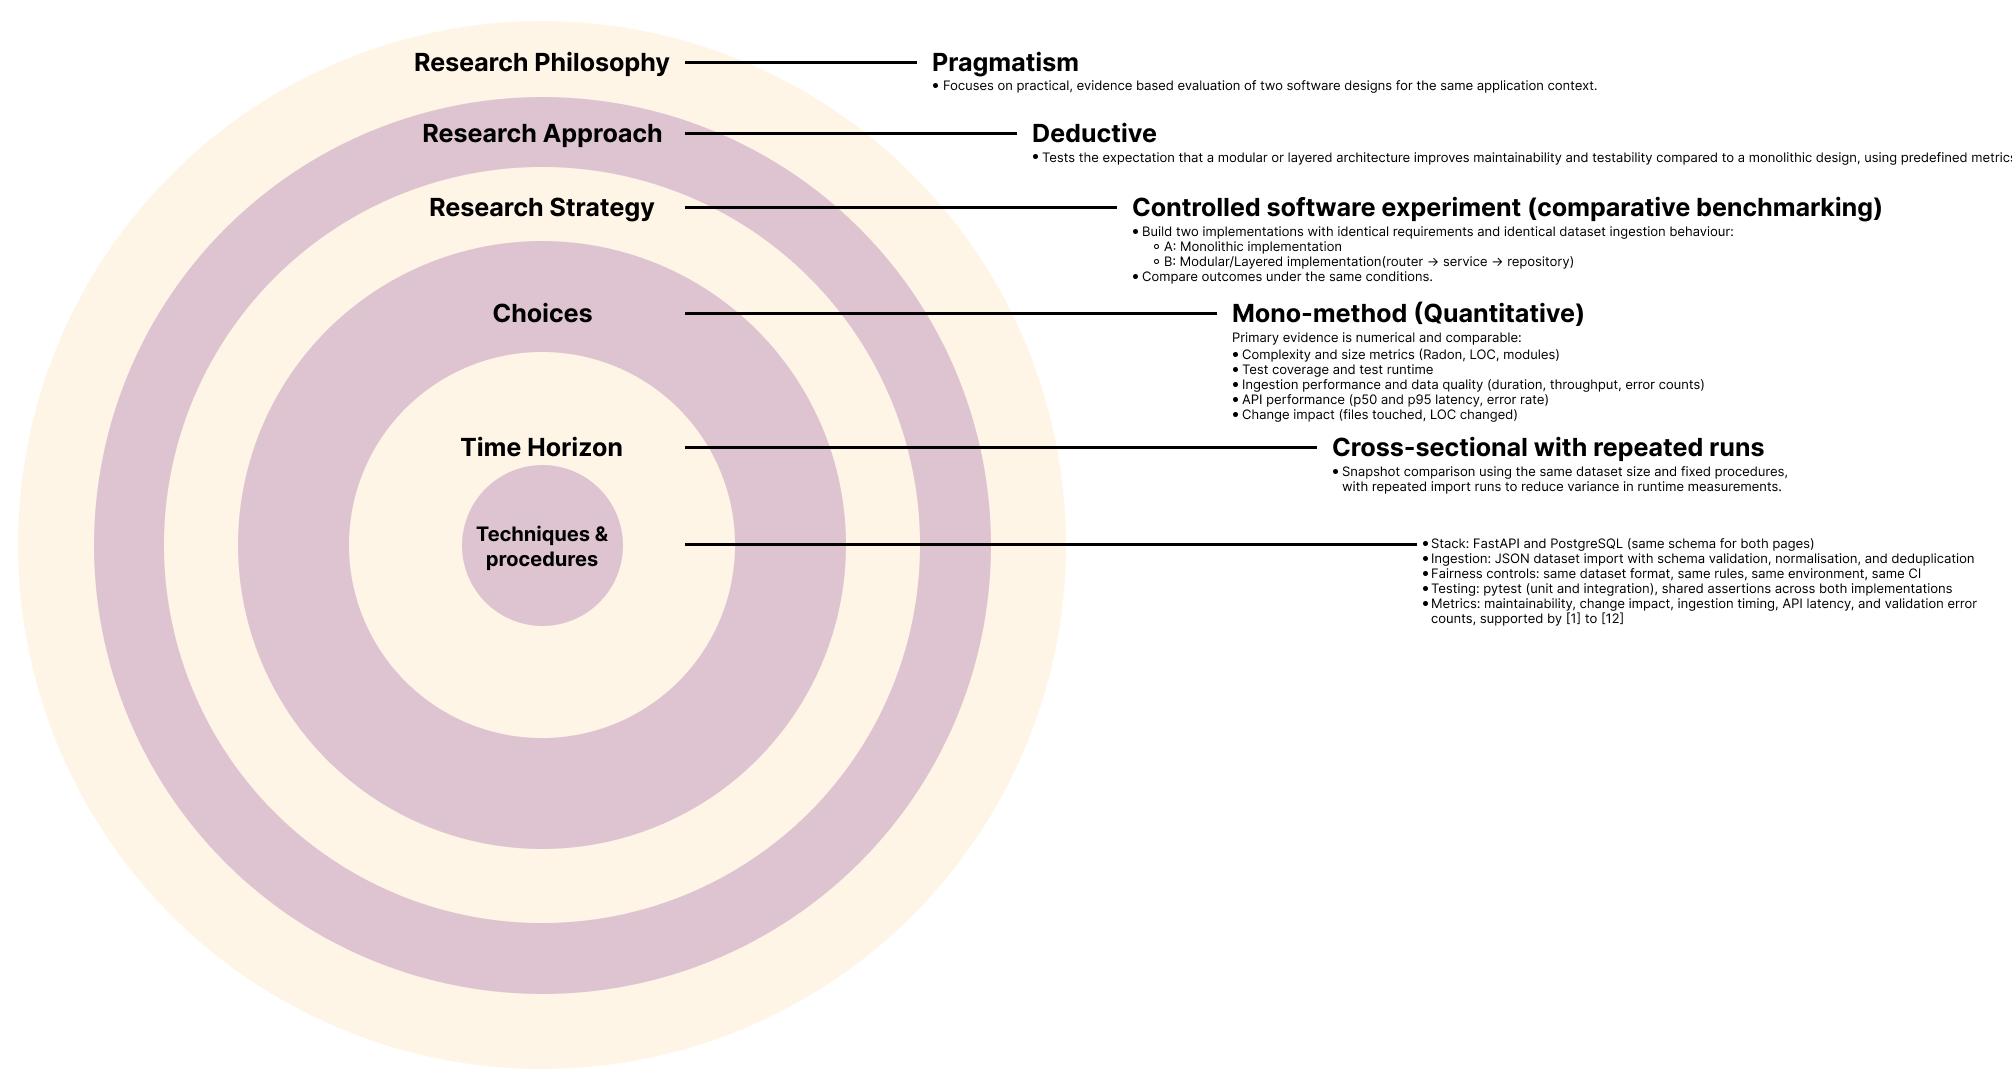
\includegraphics[width=0.75\columnwidth]{../Images/research onion.png}
\caption{Research Onion for the Study}
\label{fig:research-onion}
\end{figure}


\subsection{Background to this Research Theme}
Maintainability is widely connected to architecture quality and the presence of architectural smells. Architectural smells are recurring structures that suggest deeper design problems, and mapping studies show growing interest in their detection and management as part of controlling long term system quality [1]. Similarly, knowledge bases for architectural technical debt highlight that architecture decisions can introduce future cost, especially when system boundaries are unclear or when dependencies spread across unrelated areas [2]. Empirical work also links architectural smells to maintainability outcomes, suggesting that architecture is not only a design preference, but a factor that can affect measurable software quality [3]. 

This is relevant to the monolith versus modular discussion because a key promise of modular or layered design is that boundaries limit the spread of changes, improve test isolation, and reduce the risk that changes create unexpected side effects. Evidence on co changes and architectural smells supports the idea that when files and components tend to change together, systems become harder to evolve predictably, which motivates metrics that capture change propagation and structure quality [7]. In addition, modularity can be measured directly using modularity metrics. For example, M score is proposed as a modularity metric intended to better represent modular structure in real systems, supporting the use of modularity measurement rather than relying only on subjective judgement [8]. 

Finally, this study uses a dataset ingestion pipeline as the workload because ingestion pipelines highlight data quality issues and validation behaviour, which are important for reliability and performance. Work on data pipeline quality identifies factors and root causes that contribute to data related issues and processing problems, supporting the decision to include data quality indicators such as validation errors and duplicates as part of evaluation [5]. 


\subsection{Hypothesis, Research Aim, and Purpose Statement (including variables)}
Hypothesis: A modular or layered architecture will be more maintainable and more testable than a monolithic architecture. 

Research aim: The aim is to compare how a monolithic versus a modular or layered system design influences maintainability, testability, and operational performance in a dataset ingestion pipeline and dashboard, under controlled and identical conditions. 

Purpose statement: The purpose of this controlled comparative study is to produce measurable evidence about the impact of backend architectural structure on software quality. This is done by implementing the same case tracking application twice, once as a monolithic backend and once using a modular or layered structure, then evaluating both using the same dataset, database schema, validation rules, test suite, and runtime environment. The study also includes a controlled change request implemented in both versions to measure change impact and assess how architecture affects the effort and risk involved in evolving the system. 

Independent and dependent variables (for statistical validation):When carrying out statistical tests to validate a hypothesis, the independent variable is the factor that is deliberately changed, while the dependent variables are the outcomes that are measured and expected to change as a result. In this study, the independent variable is the backend architecture type, with two levels: (1) monolithic implementation and (2) modular or layered implementation. 

The dependent variables are the measured outcomes used to evaluate the hypothesis, including:

\begin{itemize}
\item Maintainability and structural complexity, measured using complexity and size metrics, and change impact during a controlled change request (files touched, lines of code changed, modules affected) [6], [7]. 
\item Testability, measured using unit test coverage of key ingestion and business rules, and integration test stability and runtime [11]. 
\item Operational performance, measured using import duration, throughput, validation error counts, and API latency and error rate under fixed load [5]. 
\end{itemize}

These variables allow the hypothesis to be evaluated using comparable measurements while keeping other factors controlled. 

\section{Literature Review}
This section reviews the methodologies adopted in recent studies related to software architecture quality and modularity, with a focus on how researchers evaluate maintainability, architectural smells, technical debt, and remodularisation. To provide a structured and comparative lens, this review draws upon the logic of the research onion by examining research strategy, time horizon, method choice, and evaluation procedures used to validate architecture-related hypotheses [1], [9].

Across the reviewed studies, a broadly positivist stance is evident, prioritising objective, measurable outcomes derived from software artefacts, repository history, and static analysis outputs rather than subjective judgement [1], [3], [6]. Most studies follow a deductive approach by testing expectations such as whether architectural smells relate to maintainability evidence, whether co-change behaviour aligns with architectural issues, or whether modularity can be captured through measurable metrics [3], [7], [8], [11]. The dominant strategy is empirical and observational, using smell detection pipelines, version history mining, and repeated measurement across releases, alongside supporting evidence synthesis from mapping studies and systematic literature reviews [1], [6], [9]. These methodological patterns align with cross-sectional evaluation and version-based measurement, where data is analysed at a single stage or across multiple releases to observe trends [6].

All sources in this review are academic publications, including peer-reviewed journal articles and peer-reviewed conference proceedings [1]–[12]. Non-academic material such as vendor documentation or practitioner blog posts may be useful for implementation guidance, but was not used as primary evidence here because it typically lacks clearly defined variables, reproducible evaluation, and peer-reviewed validation.

\begin{figure}[htbp]
\centering
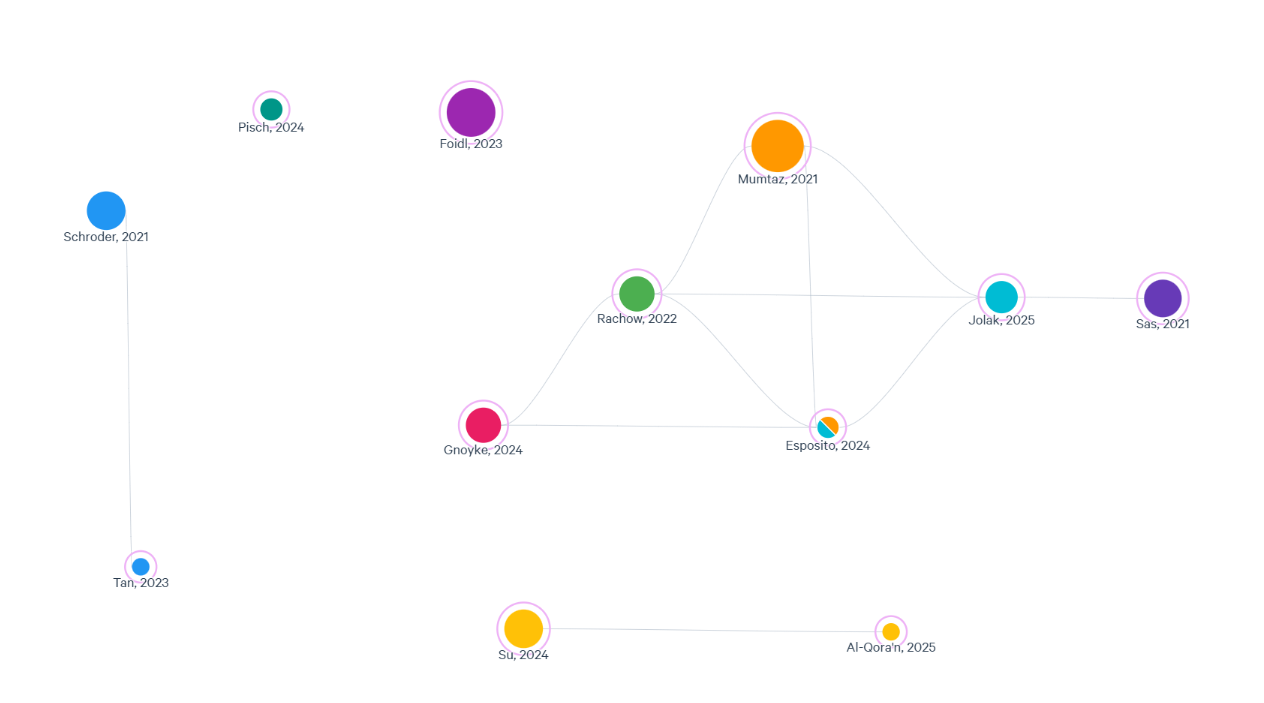
\includegraphics[width=0.75\columnwidth]{../Images/LitMap.png}
\caption{Literature Map}
\label{fig:literature-map}
\end{figure}

A literature map was constructed in Litmaps to visualise citation links between the selected academic sources [1]–[12]. Papers were grouped by concepts including smell detection and taxonomy, technical debt framing, maintainability impact evidence, smell evolution, co-change coupling, modularity metrics, modular monolith positioning, remodularisation approaches, and data pipeline quality.

Labelled relationships (conceptual legend for Fig. 2):

\begin{itemize}
\item Smell detection/taxonomy  Maintainability impact evidence: enables measurement of smells used in maintainability evaluation [1], [3], [11].
\item Technical debt (architecture)  Maintainability impact evidence: frames smells as long-term cost affecting maintainability [2], [3].
\item Smell evolution (versions)  Maintainability impact evidence: shows how smells accumulate across versions and relate to maintainability risk [6], [3].
\item Co-change/change coupling  Architectural smells: links change coupling behaviour to smell presence and architectural issues [7].
\item Modularity metric  Architecture evaluation: quantifies modular structure for comparative analysis [8].
\item Remodularisation  Modularity metric: evaluates restructuring outcomes using modularity measures and effort considerations [12], [4], [8].
\item Modular monolith (review/trend)  Architecture evaluation: positions modular monolith as a relevant approach and summarises evaluation practices [9], [10].
\item Data pipeline quality > Backend evaluation context: adds operational reliability and processing quality context relevant to ingestion-based systems [5].
\end{itemize}


\subsection{Methodologies of Similar Studies}
[1] conducts a systematic mapping study on architectural smell detection. The authors classify prior research by detection approaches, data sources, tool support, and evaluation practices. This methodology is useful for positioning because it highlights that smell detection is widely studied, but that approaches and validation methods vary across the field. The strength of [1] is the structured synthesis and clear overview of methodological trends. A limitation is that mapping studies do not directly test outcomes such as maintainability improvement, so they provide guidance on research direction rather than direct evidence for causal claims.

[3] provides an empirical investigation into how architectural smells relate to software maintainability. The methodology uses quantitative measurement, where smells are detected and then compared against maintainability-related evidence using statistical analysis. A key strength is the use of measurable variables and a repeatable pipeline. A limitation is that repository-based empirical work commonly reports associations, so maintainability differences may correlate with smells while still being influenced by other project factors.

[6] studies evolution patterns of software-architecture smells across intra- and inter-version settings. The authors use repeated measurement across many releases, which allows trends in smell appearance, persistence, and growth to be identified. This strengthens the reliability of findings compared to single snapshot studies. However, multiple factors change between versions, such as new features and refactoring, so the method is stronger for understanding evolution patterns than for proving direct cause-and-effect.

[7] explores the relationship between co-changes and architectural smells. The methodology mines version history to examine whether code entities that change together are associated with smell presence. This is relevant because frequent co-change can indicate coupling and increased maintenance effort. The strength is that it is grounded in real maintenance behaviour. The limitation is that co-change patterns can be affected by team workflow and commit practices, which may reduce internal validity if not controlled.

[8] proposes M-score, an empirically derived modularity metric. Unlike smell studies, the focus is on improving measurement quality for modular structure. This is methodologically important for architecture comparison work because modularity is often used as a dependent variable, and stronger metrics support clearer evaluation. The limitation is that modularity is multi-dimensional, so M-score should be combined with other indicators such as complexity, testability measures, and change impact evidence.

[2] introduces an architecture smell knowledge base for managing architecture technical debt. The methodology is knowledge-structuring oriented and supports decision-making by linking smells to technical debt concepts and management actions. This supports contextualisation by explaining why smells matter in practice. However, it does not provide controlled measurements of maintainability outcomes and therefore complements rather than replaces empirical evaluation.

[11] examines correlation between architectural smells and static analysis warnings. This approach strengthens evaluation through triangulation by combining architecture-level detection with independent static analysis outputs. The strength is improved construct validity. The limitation is that static warnings may vary in relevance to architecture-level quality, and correlations should be interpreted carefully.

[12] presents a search-based remodularisation case study at Adyen. The case study method provides detailed evidence in a realistic industrial context and evaluates restructuring outcomes. The strength is strong practical relevance and clear links to modularity improvement. A limitation is that findings can be system-specific and may not generalise to all domains.

[4] and [10] provide additional context. [4] proposes effort estimation for clustering-based remodularisation, contributing to how restructuring feasibility can be assessed, while [10] discusses modular monolith as an emerging trend. These sources support positioning, but provide lighter empirical evidence than journal-based studies.

Finally, [9] provides a systematic literature review of modular monolith architecture in cloud environments. This supports positioning by showing how modular monolith is defined and evaluated across studies, and highlights that methods and metrics are not fully standardised, strengthening the need for clear evaluation design in comparative work.


\subsection{Comparisons of Studies}
Across the reviewed studies, evidence synthesis papers such as [1] and [9] provide structured overviews, identifying gaps and variation in evaluation practices. In contrast, repository-based empirical studies such as [3], [6], [7], and [11] prioritise measurable indicators and tool-supported pipelines, but often provide association evidence rather than strict causal proof due to limited control over confounding variables. Case study research such as [12] provides deep contextual insight into remodularisation in practice, but can be harder to generalise across systems. These methodological differences justify the need for controlled comparative benchmarking in the current research, where requirements, dataset ingestion rules, schema, and testing conditions are kept consistent across two architecture implementations.


\subsection{Experimental Variables Used by Other Researchers}
In smell impact research, independent variables are usually smell presence, smell type, or smell intensity, while dependent variables are maintainability indicators derived from structural metrics and quality evidence [3], [6], [11]. In co-change studies, the independent variable is the co-change relationship, while dependent variables include smell presence and maintainability-related outcomes [7]. In modularity metric research, the independent variable is the modularity metric formulation, and dependent variables include modularity scores and measurement stability [8]. In remodularisation work, independent variables include the restructuring method or search strategy, while dependent variables include improvements in modular structure and effort or feasibility indicators [12], [4]. These variable choices support the structure of the current study, where architecture type is the independent variable and modularity, maintainability proxies, testability outcomes, and change impact measures are dependent variables.


\subsection{Testing Strategies Used in Related Research}
Automated smell detection pipelines with repeated extraction across versions are used in smell research, supporting repeatability but depending on tool validity [1], [3], [6]. Static analysis outputs are used for triangulation and cross-validation of quality indicators [11]. Repository mining and co-change analysis is used to test maintenance coupling using real evolution history [7]. Search-based optimisation and case study evaluation are used in remodularisation work to test whether restructuring improves modular structure, often assessed through modularity indicators and feasibility evidence [12], [4]. These strategies motivate combining structural metrics, modularity measurement, and change impact evidence for architecture comparison rather than relying on a single metric.


\subsection{Critical Synthesis and Knowledge Gaps}
The literature supports that architectural smells and technical debt are associated with maintainability risks [2], [3], [6], [11]. It also provides a range of measurement approaches, including smell detection, co-change analysis, and modularity metrics [1], [7], [8]. However, a key gap is that much empirical evidence is observational and correlational, making it difficult to isolate architectural structure as the sole cause of measured outcomes. A second gap is that modularity remains multi-dimensional, meaning a single metric cannot fully represent maintainability and testability, even when measurement quality improves [8]. A third gap is that while remodularisation case studies demonstrate practical restructuring methods [12] and effort considerations [4], there is limited controlled evidence comparing two implementations of identical requirements under identical constraints. This motivates controlled comparative benchmarking, where dataset ingestion rules, schema, API behaviour, and tests are held constant, allowing differences to be more confidently linked to architecture.


\begin{table}[htbp]
\caption{Comparative Overview of Studies}
\label{tab1}
\centering
\resizebox{1\columnwidth}{!}{%
\begin{tabular}{|c|c|c|c|}
\hline
	\textbf{Study} & \textbf{\textit{Focus}}& \textbf{\textit{Strategy \& Time Horizon}}& \textbf{\textit{Evidence Type}} \\
\hline
[1] & Smell detection research landscape & Systematic mapping, cross-sectional & Academic synthesis\\
\hline
[3] & Smells and maintainability relation & Empirical study, version-based / cross-sectional & Repository metrics\\
\hline
[6] & Smell evolution patterns & Empirical study, multi-version measurement & Repository metrics\\
\hline
[7] & Co-change and smells & Empirical study, version history mining & Repository metrics\\
\hline
[8] & Modularity measurement (M-score) & Empirical metric derivation and evaluation & Metric validation\\
\hline
[9] & Modular monolith in cloud & Systematic literature review & Academic synthesis\\
\hline
[11] & Smells and static warnings & Empirical study, cross-sectional & Smell + static analysis\\
\hline
[12] & Search-based remodularisation & Industrial case study & Applied evaluation\\
\hline
% \multicolumn{4}{l}{$^{\mathrm{a}}$Sample of a Table footnote.}
\end{tabular}%
}
\end{table}

\begin{table}[htbp]
\caption{Research design and Evaluation Tools}
\label{tab2}
\centering
\resizebox{1\columnwidth}{!}{%
\begin{tabular}{|c|c|c|c|}
\hline
	\textbf{Study} & \textbf{\textit{Research Design}}& \textbf{\textit{Data Collection}}& \textbf{\textit{Evaluation Tools / Measures}} \\
\hline
[1] & Secondary research (mapping) & Study selection and classification & Taxonomies of methods, tool support, evaluation approaches\\
\hline
[3] & Quantitative empirical & Smell detection + system measures & Statistical analysis linking smells to maintainability evidence\\
\hline
[6] & Quantitative empirical (multi-version) & Smell detection across releases & Trend and persistence analysis across intra/inter-version smells\\
\hline
[7] & Quantitative empirical & Version history mining & Co-change analysis linked to smell presence\\
\hline
[8] & Quantitative metric study & Software structure data & M-score computation, stability and modularity evaluation\\
\hline
[9] & Secondary research (SLR) & Study selection and synthesis & Comparison of definitions, evaluation practices, and gaps\\
\hline
[11] & Quantitative empirical& Smell detection + static warnings & Correlation analysis between smells and static analysis warnings\\
\hline
[12] & Industrial case study & System data from a real organisation & Search-based remodularisation outcomes, structural improvement evidence\\
\hline
% \multicolumn{4}{l}{$^{\mathrm{a}}$Sample of a Table footnote.}
\end{tabular}%
}
\end{table}


\section{Research Methodologies}
This study aims to evaluate whether a modular or layered backend architecture improves maintainability and testability compared to a monolithic backend when both implementations deliver the same application behaviour under controlled conditions. The study is applied because it produces a working software artefact and evaluates it using measurable evidence gathered from tooling, tests, and repeated benchmark runs. The methodological choices are informed by prior research on architectural smells, modularity measurement, co-change behaviour, and remodularisation, which commonly use objective, tool-supported measurements to reason about maintainability and architectural quality [1], [3], [6], [7], [8], [11].
Based on this aim, the following research questions were formed:

\hfill \break
\textbf{RQ1:} To what extent does a modular or layered backend architecture improve maintainability compared to a monolithic backend when implementing the same requirements?
\hfill \break
% \hfill \break
\textbf{RQ2:} To what extent does a modular or layered backend architecture improve testability compared to a monolithic backend under the same test suite and contract?
\hfill \break
% \hfill \break
\textbf{RQ3:} How does architecture type affect operational performance for dataset ingestion and API responsiveness under the same environment and workload?
\hfill \break
% \hfill \break
\textbf{RQ4:} How does architecture type affect change impact when implementing a controlled change request on the same codebase features?
\hfill \break

To answer these research questions, the following objectives were constructed:
\begin{itemize}
\item Implement two backend versions of the same case tracking application with identical features, API contract, database schema, and dataset ingestion behaviour.
\item Apply fairness controls by using the same dataset format and rules, the same migrations, the same environment and CI configuration, and the same shared integration tests.
\item Collect maintainability and structure evidence using tool-based metrics aligned with modularity and architectural quality research, including modularity and smell-related indicators where applicable [1], [3], [6], [8], [11].
\item Collect testability evidence using test coverage, test stability, and test execution outcomes under the same test suite and assertions.
\item Collect operational performance evidence through repeated ingestion runs and repeated API benchmark runs under the same conditions, including error counts and timing measures, informed by quality concerns in data pipelines [5].
\item Execute a controlled change request in both versions and compare change impact using measurable proxies (files touched, lines changed, and affected modules), grounded in evolution and co-change considerations [6], [7].
\item Analyse results using descriptive statistics and comparative analysis to determine whether the observed differences support the hypothesis.
\end{itemize}


\subsection{Reflection on Research Philosophy, Approach, and Paradigm}
The study adopts a pragmatist philosophy because it focuses on evidence-based evaluation of two software designs in a realistic development context. The primary contribution is practical and measurable: two working implementations are compared using consistent procedures and objective metrics rather than relying on opinion. Although many architecture studies adopt a positivist stance, pragmatism fits this work because the purpose is to support decision-making by combining software engineering measurement practices with controlled experimentation.

A deductive approach is used because the study begins with a predefined hypothesis and tests it using measurable outcomes. The hypothesis is derived from the established view in the literature that architectural structure, smells, and modularity are linked to maintainability outcomes [2], [3], [6], [11], and that modularity can be operationalised using metrics such as M-score [8]. Co-change evidence also supports the expectation that stronger boundaries may reduce change coupling and change propagation risk [7]. The study therefore tests whether the modular or layered architecture exhibits more favourable measurement outcomes than the monolith when all other factors are controlled.


\subsection{Chosen Methodology and Why It Fits the Objectives}
A controlled software experiment (comparative benchmarking) is selected as the main methodology. This choice fits the objectives because the study requires two implementations with identical requirements, followed by measurement under the same conditions so that differences can be attributed more confidently to architecture structure. This methodology also aligns with gaps identified in the literature. Many empirical studies provide strong association evidence linking architectural smells and maintainability, but they are often observational and cannot fully control confounding factors [3], [6], [11]. A controlled comparison strengthens internal validity by fixing key variables such as dataset format, schema, test suite, and environment.

The study uses a mono-method quantitative design. This is appropriate because the outcomes are defined as measurable variables such as complexity, modularity indicators, test coverage, ingestion duration, API latency, error rates, and change impact proxies. These are consistent with measurement-driven approaches seen in smell detection and maintainability research [1], [3], [6], [11], modularity metric work [8], and evolution-based change coupling research [7].

The time horizon is cross-sectional with repeated runs. Measurements are collected at a defined point when both implementations are complete, while runtime benchmarks are repeated to reduce variability in timing and throughput.


\subsection{Environment and Technologies Used}
The backend is implemented using FastAPI (Python) with PostgreSQL. The system includes a JSON ingestion pipeline that validates, normalises, deduplicates, and inserts or updates records, and records import run summaries. Both architectures implement the same endpoints and return the same responses as verified through shared integration tests. A single database schema and migration set is used for both versions to ensure fairness controls.

Tooling and evaluation procedures include:
\begin{itemize}
\item Static code and maintainability metrics (for example complexity and size indicators, and modularity indicators aligned to modularity measurement approaches such as M-score where applicable) [8].
\item Smell-oriented or architecture-quality indicators where feasible, informed by smell detection research and maintainability evidence [1], [3], [6], [11].
\item Automated unit and integration testing, with coverage reporting for unit tests.
\item Performance benchmarking for ingestion and API endpoints, including repeated-run timing and error reporting.
\item Logging and structured outputs so that results can be collected consistently across runs.
\end{itemize}


% \subsection{Equations}
% Number equations consecutively. To make your 
% equations more compact, you may use the solidus (~/~), the exp function, or 
% appropriate exponents. Italicize Roman symbols for quantities and variables, 
% but not Greek symbols. Use a long dash rather than a hyphen for a minus 
% sign. Punctuate equations with commas or periods when they are part of a 
% sentence, as in:
% \begin{equation}
% a+b=\gamma\label{eq}
% \end{equation}

% Be sure that the 
% symbols in your equation have been defined before or immediately following 
% the equation. Use ``\eqref{eq}'', not ``Eq.~\eqref{eq}'' or ``equation \eqref{eq}'', except at 
% the beginning of a sentence: ``Equation \eqref{eq} is . . .''


\vspace{12pt}
\begin{thebibliography}{00}
\bibitem{b1} H. Mumtaz, P. Singh, and K. Blincoe, “A Systematic Mapping Study on Architectural Smells Detection,” Journal of Systems and Software, vol. 173, Art. no. 110885, 2021, doi: 10.1016/j.jss.2020.110885.
\bibitem{b2} P. Rachow and M. Riebisch, “An Architecture Smell Knowledge Base for Managing Architecture Technical Debt,” in Proc. IEEE/ACM Int. Conf. on Technical Debt (TechDebt), pp. 1–10, 2022, doi: 10.1145/3524843.3528092.
\bibitem{b3} R. Jolak, S. Karlsson, and F. Dobslaw, “An Empirical Investigation of the Impact of Architectural Smells on Software Maintainability,” Journal of Systems and Software, vol. 225, Art. no. 112382, 2025, doi: 10.1016/j.jss.2025.112382.
\bibitem{b4} A. J. J. Tan, C. Y. Chong, and A. Aleti, “Closing the Loop for Software Remodularisation: REARRANGE, An Effort Estimation Approach for Software Clustering Based Remodularisation,” in Companion Proc. IEEE/ACM Int. Conf. on Software Engineering (ICSE-Companion), 2023, pp. 326–327, doi: 10.1109/ICSE-Companion58688.2023.00090.
\bibitem{b5} H. Foidl, V. Golendukhina, R. Ramler, and M. Felderer, “Data pipeline quality: Influencing factors, root causes of data related issues, and processing problem areas for developers,” Journal of Systems and Software, vol. 207, Art. no. 111855, Jan. 2024, doi: 10.1016/j.jss.2023.111855.
\bibitem{b6} P. Gnoyke, S. Schulze, and J. Krüger, “Evolution Patterns of Software-Architecture Smells: An Empirical Study of Intra- and Inter-Version Smells,” Journal of Systems and Software, vol. 217, Art. no. 112170, 2024, doi: 10.1016/j.jss.2024.112170.
\bibitem{b7} D. Sas, P. Avgeriou, R. Kruizinga, and R. Scheedler, “Exploring the Relation Between Co-changes and Architectural Smells,” SN Computer Science, 2021, doi: 10.1007/s42979-020-00407-5.
\bibitem{b8} E. Pisch, Y. Cai, R. Kazman, J. Lefever, and H. Fang, “M-score: An Empirically Derived Software Modularity Metric,” in Proc. ACM/IEEE Int. Symp. on Empirical Software Engineering and Measurement (ESEM), pp. 382–392, 2024, doi: 10.1145/3674805.3686697.
\bibitem{b9} L. F. Al-Qora’n and A. Al-Said Ahmad, “Modular Monolith Architecture in Cloud Environments: A Systematic Literature Review,” Future Internet, vol. 17, no. 11, Art. no. 496, 2025, doi: 10.3390/fi17110496.
\bibitem{b10} R. Su and X. Li, “Modular Monolith: Is This the Trend in Software Architecture?,” in Proc. 1st Int. Workshop on New Trends in Software Architecture (SATrends ’24), 2024, doi: 10.1145/3643657.3643911.
\bibitem{b11} M. Esposito, M. Robredo, F. Arcelli Fontana, and V. Lenarduzzi, “On the Correlation Between Architectural Smells and Static Analysis Warnings,” Software Quality Journal, 2025, doi: 10.1007/s11219-025-09730-7.
\bibitem{b12} C. Schröder, A. van der Feltz, A. Panichella, and M. Aniche, “Search Based Software Re Modularization: A Case Study at Adyen,” in Proc. IEEE/ACM 43rd Int. Conf. on Software Engineering: Software Engineering in Practice (ICSE-SEIP), 2021, pp. 81–90, doi: 10.1109/ICSE-SEIP52600.2021.00017.
\end{thebibliography}
% \vspace{12pt}
% \color{red}
% IEEE conference templates contain guidance text for composing and formatting conference papers. Please ensure that all template text is removed from your conference paper prior to submission to the conference. Failure to remove the template text from your paper may result in your paper not being published.

\end{document}
